\documentclass[a4paper]{article}
\usepackage[swedish]{babel}
\usepackage[utf8]{inputenc}
\usepackage[T1]{fontenc}
\usepackage{algpseudocode}
\usepackage{algorithm}
\usepackage{lmodern}
\usepackage{amsmath}
\usepackage{graphicx}
\DeclareGraphicsExtensions{.png}

\title{The Lost Vaults: Uneasy Alliance\\\small{Operativsystem och multicoreprogrammering (1DT089) våren 2013}\\\small{Slutrapport för grupp 4}}

\author{Felix Färjsjö\\(19911225-4678) \and Jimmy Holm\\(19870928-0138) \and Fredrik Larsson\\(19890422-0590) \and Anna Nilsson\\(19910804-0628) \and Philip Åkerfeldt\\(19920508-1335)}

\date{\today\\Version 1.0}

%Döp om pseudokod.
\floatname{algorithm}{Algoritm}
\renewcommand{\algorithmicindent}{4 pt}
\begin{document}
\maketitle
\thispagestyle{empty}
\newpage
\setcounter{page}{1}
\pagenumbering{Roman}
\tableofcontents
\listoffigures
\newpage
\setcounter{page}{1}
\pagenumbering{arabic}
\section{Inledning}
Att spela spel över internet har blivit en del av vår kultur som antagligen aldrig kommer försvinna. Det är ett sätt att umgås och samarbeta, ofta med människor man aldrig har mött. 
På många platser i världen är gigantiska servrar igång dygnet runt för att hantera förfrågningar från miljontals användare, och tusentals programmerare gör sitt bästa för 
att ge människor en så bra användarupplevelse som möjligt. 
För att detta ska vara möjligt krävs mycket av serverprogrammen. 
Servrarna ska kunna hantera massvis av förfrågningar med låg fördröjning, samtidigt som de måste koordinera händelser så att det som en användare gör också ska påverka dem i anslutning till den. 
Serverprogrammen ska också vara finkornigt modulariserade för att möjliggöra parallellutveckling av programmen på ett fungerande sätt.  
 
Vi kände att komplexiteten av att göra ett multiplayer onlinespel var något som utmanade och intresserade oss, då det gav upphov till intressanta problem som kunde lösas med hjälp av concurrency. 
Vi har skapat ett serverbaserat spel, som kommunicerar med användaren via en TCP/IP uppkoppling till användarens klient-program. Servern består av flera självständiga aktörer som interagerar
genom att skicka meddelanden fram och tillbaka. Detta ger oss ett bekvämt sätt att skriva fungerande spellogik, utan att behöva bry oss om att låsa delad data.

Spelet kallas \textit{The Lost Vaults - Uneasy Alliance} och är ett semi-traditionellt MUD där användaren interagerar med andra spelare och tar del i uppdrag. 
Detta sker i grupper av flertal spelare vilka tillsammans arbetar mot ett gemensamt mål. Samtidigt har varje enskild gruppmedlem en personlig agenda som endast 
gagnar den enskilda invididen. Möjligheten finns att utforska som enskild individ, men fokuset för spelet ligger i den dynamik som följer av 
interaktionen med andra spelare. Spelet utspelas på två olika platser, i City och i Dungeon. City är staden där spelarna samlas innan kommande exkursion, där kan de fylla på förnödenheter samt forma grupper för att gå ner i Dungeons. En dungeon är den värld som spelet utspelar sig i; en uppsättning rum fyllt med monster, fällor och skatter. 
Varje grupp spelare får sin egen unikt genererade Dungeon när de går ner i dessa magiska grottor under staden. Väl inne ges gruppen en eller flera uppdrag som bör fullbordas innan de kommer upp till ytan igen.

Relationen mellan konceptet concurrency och vårt projekt är förmågan att ha fler än en spelare aktiva i spelet samtidigt, samt flertalet aktiva spelområden körandes samtidigt och oberoende av varandra.

\section{Systemarkitektur}
\subsection{Design}
Systemarkitekturen som beskrivs i detta dokument är uppdelat i två delar vilka beskriver akritekturen för klienten samt servern. På grund av att både klienten och servern är skrivna i Scala och körs via Java Virtual Maschine kan de köras på alla plattformar som stödjer Java VM 1.7.
\begin{figure}[hbt]
\centering
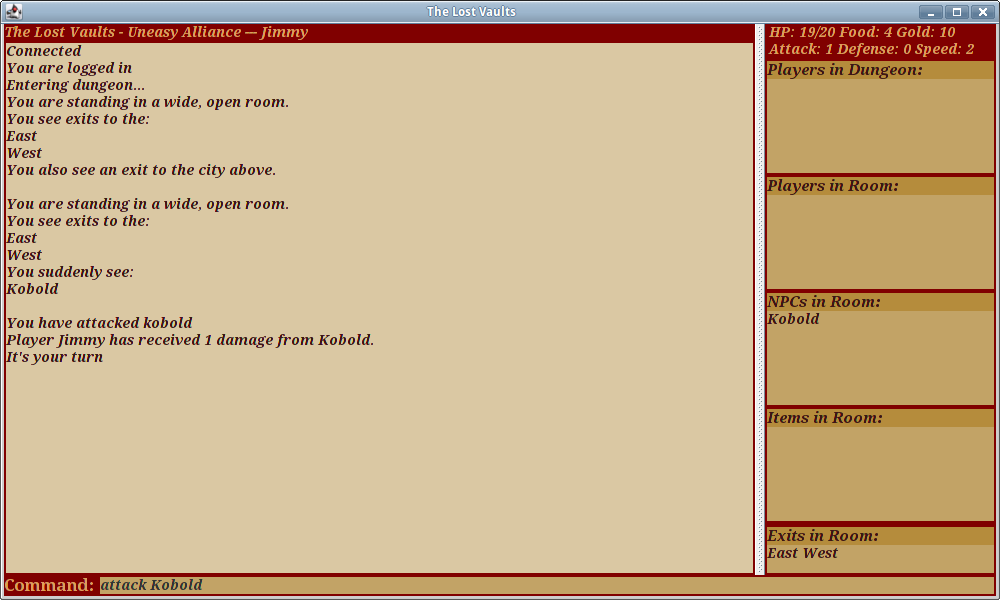
\includegraphics[width=1.0\textwidth]{client}
\caption{\label{fig:Client}Klientens användargränssnitt.}
\end{figure}

\subsection{Klient}
Designen för klienten till Lost Vaults är utvecklad för att efterlikna en indirekt terminal, vars ända uppgift är att skicka samt ta emot och tolka svaren på förfrågningar. Konceptet med en indirekt terminal valdes för att fokus skulle ligga på spellogiken, och inte på GUI:t. Det textbaserade gränssnittet tillåter utökning av serversidan utan att kräva att användaren återinstallerar sin klient. Detta innebär att det är enkelt att åtgärda buggar och bygga ut spelet utan att söra användaren. 

Klientfönstret uppdelat i flera textfält som visar relevant information för spelaren, se fig. \ref{fig:Client}. Det vänstra området är huvudområdet och används till spelets dynamiska informaton. Där får spelaren beskrivningar av rummen den besöker, meddelanden från andra spelare, meddelanden om vad som händer i spelet och liknande. Klientens högra sida innehåller statisk information som det kan vara bra för spelaren att snabbt kunna kolla upp. Den övre delen innehåller information om spelarens egen karaktär, där listas bl.a. spelarens liv, stridsegenskaper och hur mycket mat spelaren har. Den undre håller reda på vilka spelare som är i spelarens dungeon, vilka spelare som är i rummet spelaren är i, samt vad rummet har för föremål, monster och utgångar.   

Den nedre delen av fönstret innehåller kommandoraden, där spelaren skriver in kommandon i enlighet med ett strikt syntax. 

När klienten startas välkomnas spelaren av ett centrerat fönster för inloggning. Här kan spelaren skriva in sitt användarnamn och lösenord samt IP:n tillhörande den server som spelaren vill koppla upp sig mot. Lösenordet krypteras enligt SHA-256 innan det skickas över nätverket och sparas i databasen, som håller koll på användarinformationen. 

Klientens GUI är implementerat i Javas Swing UI bibliotek och integrerat i Scala för att använda Akkas TCP funktionalitet.

\begin{figure}[hbt]
\centering
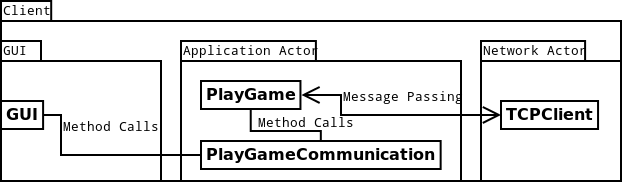
\includegraphics[width=1.0\textwidth]{clientuml1}
\caption{\label{fig:ClientArch}Klientens klassmodell.}
\end{figure}
    
\subsubsection{Klassmodell}
Klienten är strukturerad i fyra distinkta klasser, se fig. \ref{fig:ClientArch}. Klasserna PlayGame och PlayGameCommunication arbetar tillsammans för att skapa en brygga mellan TCP lagret och GUI:t. PlayGame accepterar meddelanden från TCPClient och skickar dem vidare till GUI via PlayGameCommunication. Samtidigt skickas data från GUI över nätverket via metodanrop i PlayGameCommuncation till PlayGame för att sedan hamna hos TCPClient.

\subsection{Server}
Systemarkitekturens serverdel är uppdelad i sektionerna Aktörmodell och Klassmodell. Den första delen beskriver funktionen hos de olika aktörlagren i Lost Vaults servern och den andra ger en  beskrivning av serverns klassförhållanden.

\begin{figure}[hbt]
\centering
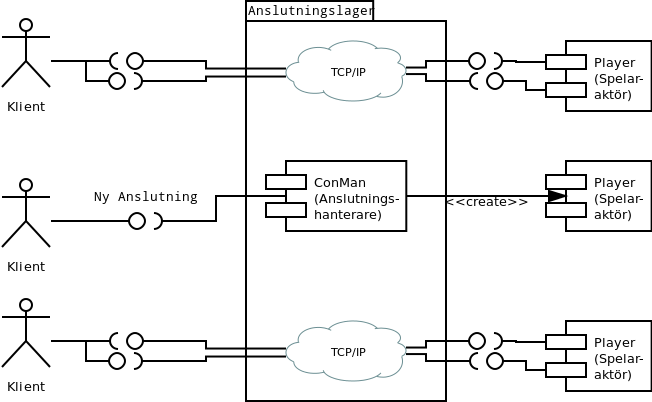
\includegraphics[width=1.0\textwidth]{serverActorModel2-1}
\caption{\label{fig:ConManPlayer}Figur över förhållandet mellan ConMan och Player.}
\end{figure}

\subsubsection{Aktörmodell}
Serverdelen är uppdelad i flera processer via Akkas aktörbibliotek för att upprätthålla Actor Concurrency-modellen .
Två typer av aktörer kommmunicerar direkt med nätverket via TCP/IP, ConManaktören och Playeraktörerna. ConManaktören har som syfte att hantera inkommande anslutningar för att sedan starta en ny Playeraktör för varje godkänd anslutning. Den nyetablerade anslutningen skickas till den nya Playeraktören, som sedan kommer hantera all kommunikation mellan spelet och den nyanslutna klienten, se fig. \ref{fig:ConManPlayer}.   

PlayerMapaktören och GroupMapaktören fyller två specifika funktioner. PlayerMap mappar på en uppkopplad spelares användarnamn till spelarens Playeraktör. Genom PlayerMap kan en aktör snabbt och enkelt skicka meddelanden till en specifik spelare baserat på dess namn - ett viktigt kommando som agerar på följande sätt är exempelvis “WHISPER”. Det är även via PlayerMap som Playeraktören ser till att samma användarnamn inte används av flera uppkopplade spelare samtidigt. 

\begin{figure}[hbt]
\centering
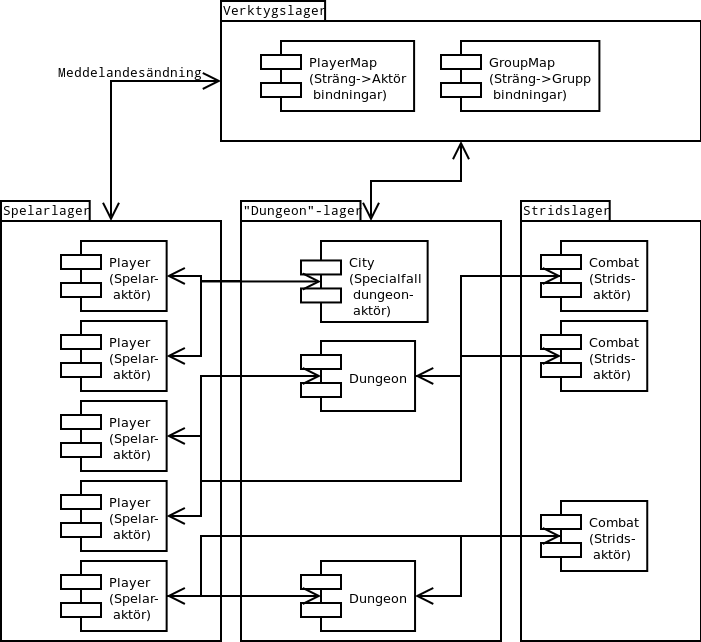
\includegraphics[width=1.0\textwidth]{serverActorModel2-2}
\caption{\label{fig:ServerActorModel}Modell över de olika aktörernas sammanhang.}
\end{figure}

GroupMapaktörens uppgift är att länka samman namn på spelare, för att forma spelargrupper, se fig. \ref{fig:ServerActorModel}. En spelargrupp är en samling av en eller fler spelare som tillsammans kan gå ner i en Dungeon. Syftet med denna aktör är att underlätta skapandet av spelargrupper samt anslutning till redan existerande spelargrupper. Genom att använda GroupMap räcker det att ansluta sig till en spelare via dess namn för att inkluderas i denna spelares grupp.

De två resterande lagren av aktörer som servern använder är Dungeonlagret och Stridslagret, och det är dessa som utför spelets logik. Det existerar ett speciellt tillstånd av Dungeonaktören, kallat Cityaktören. City är spelets uppsamlingsplats. Det är här spelaren bildar grupper med andra spelare, för att göra sig i ordning inför utforskandet av en Dungeon. Så i City kan spelaren chatta med andra spelare, köpa mat och bilda grupper.

När en grupp bestämmer sig för att stiga in i en Dungeon skapas en ny slumpvis genererad grotta, som endast de kan komma åt. Grottan består av en array med rum med dörrar som spelaren kan förflytta sig emellan. Det är i dessa rum som spelare kommer kunna göra uppdrag, finna skatter, slåss mot monster eller andra spelare etc. Dungeonaktören koordinerar också kommunikation, och händelser som påverkar spelarna som befinner sig i grottan. Ett exempel på detta är kommandot “SAY”  som skickar ett meddelande till alla spelare som är i samma rum som spelaren. 

Strider koordineras av sin egen aktör, en finit tillståndsmaskin kallad Combat, som sköter turordning av spelare och monster vid strid. Varje rum i en Dungeon kan innehålla en referens till en Combat, vilket leder till att det kan vara max en aktiv Combat per rum. Combataktören skapas då spelare går i strid mot monster eller andra spelare och terminerar när det inte längre finns någon som anfaller någon annan. 

Efter att Cityaktören har skapat en Dungeonaktör ansvarar den nya aktören för sin egen livslängd och avslutar sig själv endast när det inte längre finns några spelare i den.

\begin{figure}[hbt]
\centering
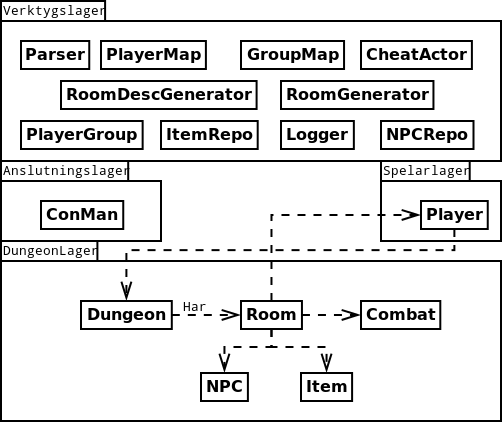
\includegraphics[width=1.0\textwidth]{serverUml2}
\caption{\label{fig:ServerKlassModell}Modell över serverns klassstruktur}
\end{figure}

\subsubsection{Klassmodell}
Klasserna i servermodellen är konceptuellt uppdelade i fyra lager: Anslutningslagret, Spelarlagret, Dungeonlagret och Verktygslagret, se fig \ref{fig:ServerKlassModell}. 

Anslutningslagret är ingångspunkten till servern över nätverket genom Akkas TCP bibliotek. Vår anslutningshanterare, ConMan, agerar som en singleton och endast en instans av denna ska existera vid en given tidpunkt. ConMan är den klass som lyssnar efter och godtar anslutningar från klienter, samt skapar nya Player-instanser vid nyupprättad anslutning. 

Dungeonlagret innehåller de klasser som är viktiga för spelets logiska funktioner. Lagret innehåller dungeonklassen, som ansvarar över en mängd slumpmässigt genererade rum. Rummen i sin tur ansvarar för aktiva strider samt icke-spelarkaraktärer och objekt. Tidigare design visar att Item klassen används som superklass till olika typer av objekt. Vi valde dock att platta till vår klasshierarki och förenkla designen genom att låta alla typer av objekt vara instanser av Item klassen med olika attribut. På samma sätt valde vi att göra oss av med distinktionen mellan goda och onda icke-spelarkaraktärer, och har istället valt att implementera enbart monster.

Verktygslagret tillhandahåller understödjande funktionalitet till de andra klasserna. Bortsett från RoomGenerator är alla klasser i Verktygslagret Singletons. 


\section{Utvecklingsverktyg}

I detta projekt användes flera olika verktyg för att underlätta utvecklingen. Då vi använt Scala som vårt val av programspråk skrevs i princip all vår kod i Eclipse. Detta då vi anser att det i särklass är det enklaste sättet att utveckla kod till Java eller Scala. Trots att all kod är skriven i Eclipse använder vi Ant Build System 
för automatiserad kompilering av vår klient och server; som sedan är klar att köras i Java Virtual Machine. 

För hanteringen av versionskontroll har vi använt det tillförlitliga och välkända verktyget Git. Vi satte upp ett nytt git repository på Github.com specifikt för detta projekt och valet av Git gjordes på grund av att vi har använt oss av det tidigare, och för att det har bra funktioner för versionshantering och för att sammanfoga parallellskriven kod. 

Testandet av vår kod görs med ScalaTest-ramverket samt ett Ant Build-skript som ger oss möjligheten till automatiskt byggande och körning av tester.

Sammansättningen av dokumentationen utförs med Scaladoc på grund av dess likhet med JavaDoc, ett verktyg vi är vana med att använda, och Ant har omarbetats för att automatiskt bygga dokumentationen.

\section{Implementation}

\subsection{Programspråk}
För att möjliggöra massiv concurrency med många individuella aktörer har vi gjort vårt projekt i Scala. Scala är bra för skalbarhet, vilket innebär att vårt program kommer fungera bra oavsätt om det är tio användare online eller om det är tio tusen. En annan anledning till att vi valde Scala är att Scala är ett objektorienterat språk, vilket passade ihop med det tänket vi hade när vi började planera programmet. Vi fokuserade på att skapa objekt som interagereade på rätt sätt med varandra, snarare än att skriva kod som ska exekveras i en särskild ordning.

Scala bygger på Java, och erbjuder därför liknande syntax. Detta innebar att övergången mellan att skriva Java och Scala var en någorlunda mjuk sådan, koden var ganska lättigenkännlig samtidigt som vi fick fördelarna med att kunna utveckla skalbart. Några nackdelar med Scala som vi finner nämnvärda är exempelvis att det, trots likheter med Java, tog en viss tid att sätta sig in i det nya 
språket vilket kan ha motarbetat utvecklingen gämfört med om vi hade valt ett annat språk som vi var mer bekanta med.

Genom rekommendationer av skaparna bakom Scala, beslöt vi oss för att använda Akka som vårt aktörbibliotek. Detta för att kunna använda Akkas TCP-bibliotek för nätverkskommunikationen. Bibliotekets enkla integration var en av punkterna som ledde till vårt beslut att använda Scala och Akka som val av programspråk och aktörbibliotek.

Java var det språket vi valde att använda vid skapandet av det grafiska gränssnittet som spelaren agerar mot. Vårt val grundade sig i biblioteket Swing som Java tillhandahåller. 
Med hjälp att detta bibliotek var skapandet av det grafiska gränssnittet en relativt enkel process. Likt många andra av Javas bibliotek var dokumentationen välskriven och enkel 
att använda vilket underlättade processen. En annan aspekt som fick oss att välja Java för just denna del var att vi ville kunna kommunicera med resterande kod, skriven i Scala, 
på ett enkelt sätt och detta kunde uppnås utan problem då Scala är byggt utifrån Javas Virtuella Maskin. 

\subsection{Algoritmer}
För att spelarna alltid skall få  nya och intressanta upplevelser bestämde vi oss för att skriva en algoritm för slumpmässig generering av rum som spelarna kan utforska. Vi
bestämde oss för att nyttja ett rutnät där varje cell representerar ett rum. Spelare kan ta sig från rum till rum via utgångar placerade på några av eller alla rummens fyra väggar.
Vår algoritm skall även säkerställa att inga rum skapas som inte går att nå från ingången. Nedan beskrivs med pseudokod den algoritm vi bestämde oss för att använda. I kort fungerar algoritmen så att först slumpas koordinaterna till ett rum som blir startrummet. Därefter slumpas koordinaterna till ett annat rum varefter programmet går i slumpad riktning från det nya rummet till angränsande rum, samtidigt som nya rum skapas i varje ny besökt koordinatruta, tills det nya rummet har fått en anknytning till startrummet.
\begin{algorithm}
\caption{Procedurell Rumsgenerering.}
\label{alg:RoomGen}
\begin{algorithmic}[1]
\Function{generateRooms}{Bredd, Höjd}
\State  $Rooms$ = Array[Bredd * Höjd]
\State  $StartRoom$ = slumpmässig cell i $Rooms$
\State  $CreatedRooms$ = $0$
\State  $GoalRooms$ = önskat antal skapade rum
\Repeat
\State $ToConnect$ = List()
\State $NextRoom$  =  Slumpat rum $x$ ur $Rooms$ där $x.created = false$
\State $NextRoom.created$ = $true$
\State $ToConnect.Insert NextRoom$
\While{$NextRoom.connected \neq true$}
\State Välj en slumpmässig riktning, viktad mot $StartRoom$
\State $NextRoom$ = den cell i $Rooms$ som är ett steg i vald riktning
\If {$NextRoom.created = true$ och $NextRoom.connected \neq true$}
\If {Andra riktningar har inte prövats}
\State Välj ny riktning och börja om från $13$
\ElsIf{Alla riktningar har misslyckats}
\State Gå tillbaka ett rum ur $ToConnect$ och börja om från $12$
\If{Alla möjliga riktningar prövats i alla rum ur $ToConnect$}
\State Börja om från $7$
\EndIf
\EndIf
\ElsIf{$NextRoom.created = false$}
\State Lägg $NextRoom$ först i $ToConnect$
\EndIf
\EndWhile
\While{$|ToConnect|$}
\State Anslut $NextRoom$ med $ToConnect$
\State Sätt $NextRoom.connected = true$
\State Plocka ut $head$ från $ToConnect$ och tilldela den till $NextRoom$
\State Öka $CreatedRooms$ med $1$
\EndWhile
\Until{$CreatedRooms \geq GoalRooms$}
\EndFunction
\end{algorithmic}

\end{algorithm}

\subsection{Datastrukturer}

\subsection{Concurrency}
Flera spelare samtidigt
Skicka meddelanden - jobbigt när man bara vill ta reda på ett värde - skicka meddelanden fram och tillbaka. Men ingen risk för deadlock då all kommunikation sker via meddelanden. 
Meddelanden är ej synkrona, vilket märks då en spelare ibland kan bli slagen efter att den har dött (det ser uut så i prompten eftersom meddelandena kommer så, men det är inte sant)
För att skapa en slags synkronisering har vi använt FSM, vilket kräver att man är i en särskild state för att kunna ta emot ett särskilt meddelanden. 

\section{Slutsatser}
Vårt slutresultat är ett textbaserat multiplayer dungeon spel. I spelets startrum kan man chatta med de andra spelarna som är online genom \textit{WHISPER} (personligt meddelande) eller \textit{SAY} (till alla spelare i rummet). Där kan man också forma en grupp så att man tillsammans med andra spelare kan gå ner i en dungeon och börja spela. Väl nere i en dungeon kan man chatta som vanligt, men man kan också plocka upp saker man hittar, gå till andra rum och slåss mot andra spelare eller NPC som är i rummet. När detta sker uppdateras klienten på korrekt sätt, så att spelaren får information om vad som händer i grottan.

Vi har också skapat ett administrationsverktyg som gör att man i terminalen kan ge spelare objekt, återställa hälsan så att spelaren får fullt HP\footnote{HP står för Health Points, vilket är hur mycket liv spelaren har vid givet tillfälle} och skada den genom att bestämma hur mycket HP som ska dras av (man kan inte döda en spelare). Detta gjorde vi för att kunna testa spelet och för att kunna visa upp hur det faktiskt fungerar utan att behöva leta genom alla salarna.     

Något vi gjorde bra var att vi gjorde klart det essentiella för huvudmålet med projektet, att uppnå concurrency på något sätt. Spelet hanterar många individuella aktörer, och klarar av att hantera massiva uppkopplingar mot dess server. 
Då den delen av projektet var klart kunde vi utöka produkten med funktioner för att göra spelet roligare och mer interaktivt. 
Implementation av föremål och monster att slåss mot i grottan. 
Något vi lärt oss är att skriva nätverkskod. Vi har även fått kunskap i ett nytt programspråk.
Det vi tycker har varit svårt var bland annat att integrationstesta våra aktörer. Svårigheterna uppstod på grund av bristande 
information att ta del av om hur vi skulle gå till väga för att göra detta. En annan sak som också varit relativt svår var att 
begränsa oss när det gällde den utsträckning för vilket spelet skulle utvecklas. Att begränsa utvecklingen till en rimlig nivå för spelet 
och samtidigt ha det tillräckligt intressant för den som spelar.

En stor sak som vi inte hann med under projektets gång är att implementera uppdrag. Utan uppdrag missar spelet sitt djup, och lyckas inte fånga spelaren. Dessutom ska spelet ha fällor i vissa rum, för att göra färden genom grottorna farligare. 

Vi har arbetat med automatiserad testing medan vi har byggt upp vårt spel. Men på grund av aktöruppbyggnaden av vårt program har det vara svårt att göra annat än enhetstester, och dessa har endast gett ytlig testning av spelet, då mängder av olika händelseförlopp kan inträffa. Så för att uppväga våra brister i automatiserade tester har vi helt enkelt testkört spelet många gånger. 



\section{Appendix}

Scala 2.10.4, Akka 2.3.2, SLF4J 1.7.7, Slick 2.0.2, SQLite JDBC 3.7.2

https://github.com/senilica/LostVaults/

Vilka versioner av till exempel Erlang, Java, Python etc har använts?
Hur kan koden laddas ner? Finns koden tillgänglig på till exempel GitHub eller Bitbucket eller som Tar arkiv?  Beskriv projektets katalogstruktur.
Vilket stöd för automatiserad testning finns och hur används det, till exempel JUnit (Java), EUnint (Erlang) eller PyUnit (Python)?
%Vilket stöd för automatiserad generering av dokumentation finns och hur används det, till exempel Doxygen (C, C++, C\#, Fortran, Java, Objective\­C, PHP, Python), EDoc (Erlang), Pydoc (Python), Javadoc (Java)?
Hur kompileras systemet?
Hur startas systemet? tryck på play


\end{document}
